\section{Formulación del problema}
¿Cómo se puede mejorar la comprensión oral del idioma inglés para la población bilingüe en Colombia?.
\medskip

\section{Descripción del problema}
América latina, se ubica por debajo del promedio mundial en el EF English First Proficiency Index (EF EPI) en todos los grupos de edad \cite{icfes2022informe}, los gobiernos latinoamericanos reconocen la importancia que tiene el inglés y realizan diferentes estrategias para brindar el aprendizaje del lenguaje, sin embargo, al ser una lengua extranjera se convierte en un reto el aplicar los conocimientos adquiridos, esto lo vemos reflejado en el dominio del inglés de la población latinoamericana que, si bien han pasado por procesos de aprendizaje, al no mantener y/o establecer una cultura bilingüe, tienden a descuidar sus conocimientos en este lenguaje, presentando una pérdida de oportunidades laborales e inclusive académicas, ya que el inglés, al ser uno de los lenguajes más utilizados en el mundo, ha sido incluido en diversos proyectos, investigaciones, entretenimiento e inclusive herramientas de trabajo, con lo cual, al no contar con diferentes espacios para la práctica del idioma extranjero, se perderán diversas oportunidades para crecer profesional y académicamente. Una de las principales causas es la falta de escenarios para poder practicar un segundo idioma como el inglés, este es un reto por el cual por más que una persona ingrese a un plan de enseñanza ya sea por medio de alguna institución o a través de cursos gratuitos en internet, al vivir un entorno en monolingüismo, se presenta un nivel de apropiación del idioma bajo, haciendo que los únicos lugares en donde se haga uso de una segunda lengua sea solo dentro de las instituciones de enseñanza o dentro de algunos lugares de trabajo, según políticas de cada empresa \cite{cronquist2017aprendizaje}.
\\
\\
En Colombia existen 2 calendarios escolares (Calendario A y Calendario B),  los jóvenes cursantes del último año de bachillerato deben de enfrentarse a una prueba en la cual mide su nivel de aprendizaje durante todo el ciclo escolar, este tiene como nombre examen Saber 11°, el cual tiene una prueba incluida sobre los conocimientos aprendidos en un segundo idioma, el inglés. En 2020 para el calendario A el puntaje promedio de los estudiantes que tomaron el examen fue de 48 puntos y para el calendario B los estudiantes sacaron un puntaje de 72 puntos, algo a tener en cuenta es que los estudiantes del calendario A en un intervalo de tiempo del 2018 hasta 2020 presentaron un comportamiento decreciente, pues en el año 2018 se obtuvo un promedio de 52 puntos. \cite{icfes2022informe} Para el Calendario B en un intervalo de tiempo del 2017 hasta 2020 presentó una tendencia creciente al pasar de 70 a 72 puntos. En ambos casos los resultados dejan mucho que desear pues la prueba icfes tiene como fin evaluar a los estudiantes con una prueba de inglés la cual evalúa su conocimiento  hasta B + (más allá de B1 pero sin llegar a B2)\cite{molina2021gamificacion}, además es un punto crucial ya que la gran mayoría de las personas en colombia por cuestiones económicas y/o sociales no tienden a adquirir más conocimiento sobre este idioma ya sean cursos o instituciones. Estos resultados implican muchas variables como el contexto social en el que vive el estudiante, el nivel de apropiación de las instituciones, métodos de enseñanza que el colegio posee para que sus estudiantes logren obtener un buen aprendizaje (los cuales la mayoría tienden a ser monótonos y ortodoxos ). Como se puede ver en la Figura 1(Árbol de problemas), La ausencia de un enfoque centralizado del uso de la IA para la enseñanza del inglés es un problema que implica el mejoramiento del aprendizaje de este idioma, desaprovechado las técnicas de IA disponibles en el mercado se pierde la innovación que pueden traer la implementación de estos modelos matemáticos en la enseñanza de idiomas y, al no contar con estas herramientas se reduce la eficacia del aprendizaje, y esto se refleje en una pérdida de oportunidades tanto académicas como profesionales.
\\
\\
\begin{figure}[H]
    \centering
    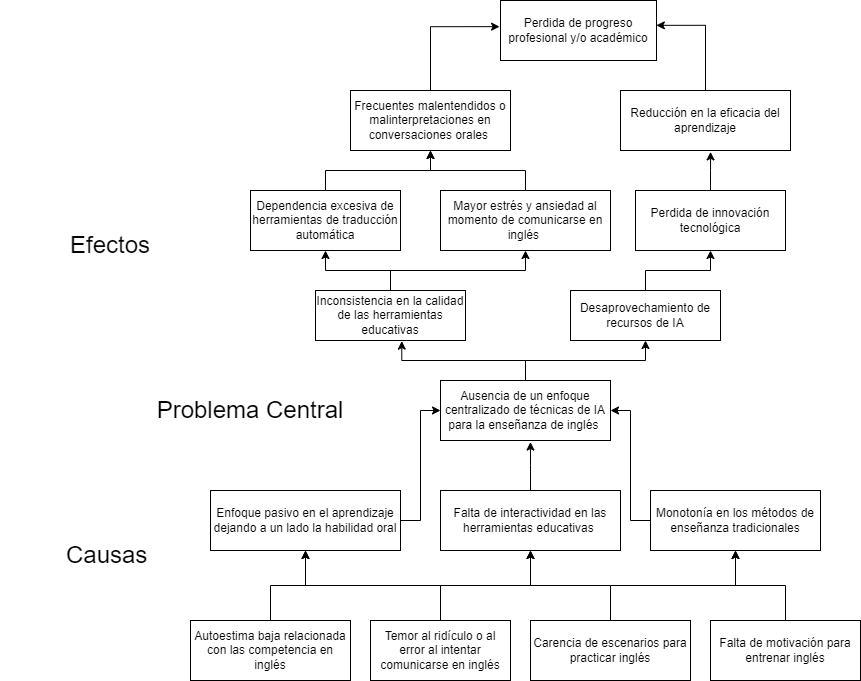
\includegraphics[width=1\linewidth]{Imagenes/seminario Arbol de problemas.png}
    \caption{Árbol de problemas}
    \label{fig:enter-label}
\end{figure}





 
 

